% NO NEED TO CHANGE ANYTHING IN THIS FIRST LINE
\documentclass[aps,prl,twocolumn,groupedaddress]{revtex4}

% INCLUDE PACKAGES

% -- THIS PACKAGE WILL LOAD GRAPHICS HANDLING FUNCTIONALITY
\usepackage{graphicx}

% DEFINE COMMANDS

% -- THIS COMMAND CREATES A SHORTHAND FOR \begin{equation}
\newcommand{\beq}{\begin{equation}}
% -- THIS COMMAND CREATES A SHORTHAND FOR \end{equation}
\newcommand{\eeq}{\end{equation}}
% -- THIS COMMAND TAKES ONE ARGUMENT AND PLACES IT INSIDE OF PARENTHESIS
\newcommand{\of}[1]{\left(#1\right)}

\begin{document}


\title{Determining maximum power output of cantilever based Piezoelectric Energy Harvester under various resonant conditions}


\author{Kurt VonEhr}
\email[]{vonehrk@gvsu.edu}
\affiliation{ Padnos College of Engineering and Computing, Grand Valley State University}

\date{\today}

\begin{abstract}

Piezoelectric devices will produce varying outputs (voltage, current, etc) depending on the resonance of their structure. For this experiment, the structure under study will be a single bimorph piezocantilever containing a steel sheet metal substrate. Without performing a complex mathematical analysis of the systmem, a rough optimization of a piezoelectric cantilever harvesting system can be obtained through experimentation. In this experiment, the maximum power output of the energy harvesting device will be determined by measuring the charge accumlated on a storage capacitor of known capacitance, after a consistent number of plucks and pluck angle for each particular resonant configuration. The resonsance will be varied by moving a tip mass to different positions along the cantilever arm. The cantilever substrate will be assumed to be massless with respect to the tip mass. The results should illustrate which length will maximize the power output of the cantilever arm when plucked. This experimentation is necessary in order to prototype design a roughly optimized Harvesting Node Device (HND). This device will contain 12 cantilever harvesting arms and be used to transmit data. The HND is the driving motivation of this experiment. 
\end{abstract}
 
\maketitle

\section{Procedure}

Due to the unique structure of the desired HND (not in the scope of this report), a non commercially available piezo cantilever device must be constructed. A piezo sheet of size 2.85in x 2.85in was purchased and is the starting point for the piezo dimension choices. The design of the HDN will include 12 bimorph cantilevers. To optimize the available piezo material for 12 cantilevers,  the dimensions of each bimorph structure will be as shown in FIG. 1. The values of X1 and X2 shown in FIG. 1, will be varied individually, such that the particular lengths can be isolated and the associated generated charge measured. To ensure that the generated power is consistant, the angle of the pluck release will be held constant. The angle will be loosely based upon the commercial product manufactered by Volture, who lists a maximum tip to tip displacement of .12in for the V22BL model \footnotemark\footnotetext{\url{http://www.mide.com/pdfs/Volture_Datasheet_001.pdf}}. The distance from base to tip is 2.75in. The angle of displacement is therefore: 

\begin{equation}
 2.49 ^\circ = \arctan (.12/2.75)
\end{equation}

\begin{figure}[ht!]
  \centering
  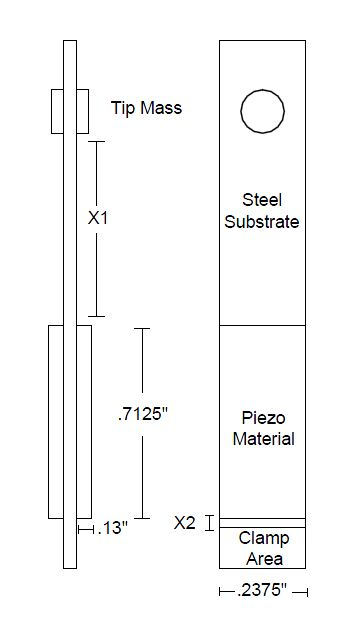
\includegraphics[scale=0.6]{Bimorph_Cantilever.jpg}
  \caption{Laboratory Test Bimorph Piezoelectric Cantilever}
\end{figure}

Using this angle (1) as a reference and prior knowledge of the bimorph cantilever, an angle of $3^\circ$ will be used. In previous experiments, the cantilever was allowed to bend further than $2.5^\circ$ without damage. The sheet will be cut by razo blade etching and a controlled break as indicated on this webpage: \url{http://www.piezo.com/tech3faq.html}


Finally, the transistor maintains a fixed voltage between the base and the collector.  Referred to as $V_{be} \equiv V_b - V_e$, this value is approximately 
\begin{equation}
	V_{be} \approx 0.6 \, V \, .
	\label{eq:transistorlinear3}
\end{equation}
The three equations~\ref{eq:transistorlinear1}, \ref{eq:transistorlinear2}, and \ref{eq:transistorlinear3} may be used to analyze a transistor operating in the linear regime. 

The transistor will not operate as described above if $I_b$ becomes too large.  When this happens the transistor is said to be \emph{saturated} and  $\beta$ is no longer constant.  When the transistor is saturated the voltage difference between the collector and the emitter drops to $V_{ce} \equiv V_c - V_e \approx 0.1$--$0.4 V$  while for a transistor operating in the linear regime this difference is always at least as big as $V_{be}$ so that the voltage hierarchy $V_b > V_c > V_e$ is preserved. The experiment performed here will provide a quantitative measure of how large $I_b$ needs to be to drive the transistor into saturation mode.



% THE NEXT SECTION IS THE PROCEDURE
\section{Procedure}

The circuit used to determine $\beta$ for the 2N2222 transistor is shown in Figure~\ref{fig:circuit}.  The base current $I_b$ is controlled by the variable resistor $R$.  Applying Ohm's Law to the base leg of the circuit gives 
\begin{equation}
	5 \, V - I_b \, R - I_b \, 4.7 \, \mathrm{k}\Omega = V_b \, . 
	\label{eq:OhmBase}
\end{equation}
Equation~\ref{eq:transistorlinear3} applies to both the linear and saturated regimes and we therefore expect the base-emitter voltage difference of the transistor to be $V_b - V_e \approx 0.6 \, \mathrm{V}$.  Combining this with Equation~\ref{eq:OhmBase} we see that the base current will be given by
\begin{equation}
	I_b = \frac{4.4 \, V}{R + 4.7 \, \mathrm{k}\Omega} \, .
	\label{eq:Ibcalc}
\end{equation}
The experiment is set up so that we will measure the collector current $I_c$ directly.  We can use this to determine the value of $V_c$ by applying Ohm's Law to the collector leg of the circuit:
\begin{equation}
	+12 \, V - I_c \, R = V_c \, . 
	\label{eq:Vccalc}
\end{equation}



\section{Results}

The collector current $I_c$ was measured for a range of resistor values $R$ between $0$ and $1 \, \mathrm{M}\Omega$.  The results are shown in Table~\ref{tab:data}.  For each value of $R$, $I_b$ was calculated using Equation~\ref{eq:Ibcalc} and $V_c$ was calculated using Equation~\ref{eq:Vccalc}.  From the measured value of $I_c$ and the calculated value of $I_b$, $\beta$ was calculated according to Equation~\ref{eq:transistorlinear1}.

% HERE WE INCLUDE A TABLE.  THE [h] COMMAND HAS THE SAME EFFECT AS IN THE
% FIGURE ENVIRONMENT ABOVE
\begin{table}[h]
	% THE CAPTION COMES FIRST FOR A TABLE
	\caption{Experimental data.  For each value of the variable resistor $R$, the collector current $I_c$ was measured, and the collector voltage $V_c$, base current $I_b$ and proportionality constant $\beta$ were calculated according to Equations~\ref{eq:Vccalc}, \ref{eq:Ibcalc}, and \ref{eq:transistorlinear2} respectively. }
	% NEXT A RULEDTABULAR WILL PLACE DOUBLE LINES ABOVE AND BELOW THE TABLE
\begin{ruledtabular}
	% THIS COMMAND ACTUALLY BEGINS THE TABLE.  THE COMMAND {ccccc} TELLS LATEX 
	% THAT THIS TABLE HAS FIVE CENTERED COLUMNS.  THE COMMAND {crl} WOULD 
	% PRODUCE THREE COLUMNS.  THE FIRST CENTERED, THE SECOND RIGHT-JUSTIFIED,
	% AND THE THIRD LEFT-JUSTIFIED
	\begin{tabular}{ccccc} 
	% FOR EACH ROW, THE ELEMENTS ARE SEPARATED BY &.  THE COMMAND \\ ENDS A 
	% ROW AND A \hline COMMAND CAN BE USED TO DRAW A HORIZONTAL LINE SEPARATING 
	% THIS ROW FROM THE NEXT
	$R \, \of{\mathrm{k} \Omega}$ & $I_c \, \of{\mathrm{m} A}$ & $V_c \, \of{V}$ & $I_b \, \of{\mathrm{m} A}$ & $\beta$ \\  \hline
	0 & 11.67 & 0.04 &  0.94 &  12.4 \\ 
	47 & 11.54 & 0.17  & 0.09  & 130 \\ 
	100 & 8.33 & 3.3  & 0.04  & 189 \\ 
	470 & 1.90 & 9.78  & 0.01  & 196 \\ 
	1000 & 0.9 & 10.75  & 0.005  & 196 \\ 
	\end{tabular}
	\end{ruledtabular}
	% AGAIN A LABEL IS PROVIDED SO THAT THIS TABLE CAN BE REFERENCED
	\label{tab:data}
\end{table}





Figure~\ref{fig:betavsR} shows a plot of $\beta$ versus the resistance $R$.  For values of $R$ of $100 \, \mathrm{k}\Omega$ and above, the transistor is clearly operating in the linear regime and $\beta$ is approximately constant and equal to $\beta \approx 190$.  From Table~\ref{tab:data} we see that these values of $R$ correspond to base currents of $I_b < 50 \,  \mu A$.  We also see from Table~\ref{tab:data} that for these values of $R$ the voltage hierarchy is satisfied with $V_c > V_b = 0.6 \, V$.




% THE FINAL SECTION IS DISCUSSION
\section{Discussion}

This experiment has shown that the 2N2222 transistors operate in the linear regime for base currents of $I_b < 50 \, \mu A$ and that for base currents in this range the voltage hierarchy is satisfied.  When operating in the linear regime, it has been verified that the base and collector currents are proportional with $\beta \equiv I_c/I_b \approx 190$.  

The experiment could have been improved by measuring the actual voltage of the $+12 \, V$ and $+5 \, V$ terminals, and by directly measuring the voltage difference $V_{ce}$ between the collector and the emitter. Since our determination of $I_b$ (and therefore $\beta$) relied on knowledge of these values, it would have been preferable to measure them directly.

\vfill


% THE FOLLOWING COMMAND WILL CREATE THE BIBLIOGRAPHY.  THE THING THAT GOES IN
% PARENTHESIS IS THE NAME OF YOUR .bib FILE WITHOUT THE .bib EXTENSION
\bibliography{samplelab}

\end{document}
%
% ****** End of file template.aps ******
